\documentclass[oneside,final,12pt]{extreport}
\usepackage[utf8]{inputenc}
\usepackage[T2A]{fontenc}
\usepackage{vmargin}
\usepackage[english, russian]{babel}
\usepackage{indentfirst}
\usepackage{amsmath}
\usepackage{filecontents, pgfplots}
\usepackage{caption}
\usepackage{tikz}
\usepackage{float}
\usepackage{amsthm}
\usepackage{amssymb}
\usepackage{amsfonts}
\usepackage{verbatim}
\usepackage[framed,numbered,autolinebreaks,useliterate]{mcode}

\usepackage{fancyvrb}
\setpapersize{A4}
\setmarginsrb{2cm}{1.5cm}{1.5cm}{2cm}{0pt}{0mm}{0pt}{13mm}
\usepackage{listings}

\definecolor{myblack}{rgb}{0,0,0}

\lstset{
	keywordstyle=\color{myblack},
	stringstyle=\color{myblack}
}

\newtheorem{theorem}{Теорема}

\renewcommand{\thechapter}{\arabic{chapter}.}
\renewcommand{\thesection}{\arabic{section}.}

\newenvironment{compactlist}{
  \begin{list}{{$\bullet$}}{
    \setlength\partopsep{0pt}
    \setlength\parskip{0pt}
    \setlength\parsep{0pt}
    \setlength\topsep{0pt}
    \setlength\itemsep{0pt}
  }
}{
  \end{list}
}

\begin{document}
	\begin{titlepage} 
		\begin{center} 
		
			
\includegraphics[width=55mm]{msu} 
			\line(1,0){400}
		
			Московский государственный университет имени М.В.~Ломоносова\\ 
			Факультет вычислительной математики и кибернетики\\ 
			Кафедра оптимального управления 
		
			\vspace{3.5cm} 
		
			{\Large Отчет по практикуму}
		
			\vspace{1cm} 
		
			{\Large{\textbf{Программа для решения краевых задач методом продолжения по параметру\\}}}
		
		\end{center} 
	
		\vfill 
	
		\begin{flushright} 
			\textbf{Студент}\\ 
			313 группа \\ Мнацаканян Шант Атомович
		\end{flushright}
	
	%		\vspace{0.1cm}
	
		\begin{flushright} 
			\textbf{Преподаватели}\\ 
			Киселёв Юрий Николаевич\\
			Аввакумов Сергей Николаевич\\
			Будак Борис Александрович\\
			Груздев Арсений
		\end{flushright} 
	
		\vfill 
	
		\begin{center} 
			Москва, 2017 
		\end{center} 
	
		\enlargethispage{4\baselineskip} 
	
\end{titlepage}

\setcounter{page}{2}
\tableofcontents

\chapter*{О проекте}
\addcontentsline{toc}{chapter}{О проекте}

\section*{Цель проекта}
\addcontentsline{toc}{section}{Цель проекта}

Реализовать программу в среде \textit{Matlab}: программа для решения кравевых задач методом продолжения по параметру и отображения результатов работы в виде графиков и таблиц.

\section*{Используемые объекты}
\addcontentsline{toc}{section}{Используемые объекты}

Программа реализована в среде \textit{Matlab 2016b}. Использовались всевозможные средства среды для реализации пользовательского интерфейса, аналитического решения возникающих задач, чтения и записи файлов.\\ 


\section*{Описание программы}
\addcontentsline{toc}{section}{Описание программы}

Программа имеет многооконный интерфейс. Основное окно программы содержит четыре блока элементов интерфейса.

Первый блок, меню в верхней части окна, имеет четыре пункта. В первом пункте собраны команды для сохранения введённой задачи (<<Сохранить задачу>>, комбинация горячих клавиш \textit{Ctrl+S}), которая открывает стандартное системное окно сохранения файлов, загрузки ранее введённой задачи (<<Загрузить задачу>>, комбинация горячих клавиш \textit{Ctrl+O}), которая открывает стандартное системное окно открытия файлов и выхода из программы (<<Выход>>, комбинация горячих клавиш \textit{Ctrl+Q}), которая либо открывает диалоговое окно с предупреждением, если задача не сохранена, либо закрывает программу. Второй пункт меню открывает окно с библиотекой примеров (<<Библиотека примеров>>, комбинация горячих клавиш \textit{Ctrl+L}), в котором представлен список примеров из учебного пособия [5], а так же присутствуют две кнопки для открытия примера и закрытия окна. Третий пункт меню открывает окно Помощь (<<Помощь>>, комбинация горячих клавиш \textit{Ctrl+H}). Четвёртый пункт меню открывает окно О программе (<<О программе>>, комбинация горячих клавиш \textit{Ctrl+A}).

Второй блок, блок для введения системы дифференциальных уравнений и краевых условий, содержит две таблицы, в которые необходимо вводить саму краевую задачу. Размерность таблиц регулируется автоматически, новые поля появляются при необходимости.

Третий блок, блок для настроек метода, содержит поля для ввода начала отрезка, конца отрезка, количества итераций, точности для внешней задачи, точности для внутренней задачи, метода решения для внешней задачи, метода решения для внутренней задачи, шага сетки, выбора точки $t_*$ и ввода вектора начальных условий $p_0$.

Наконец, четвёртый блок содержит три кнопки для решения введённой задачи, удаления решения и открытия окна с результатами. 

Окно <<Результаты>> содержит пять блоков элементов интерфейса. 

В первом блоке в меню присутствует команда для закрытия окна. 

Второй блок содержит координатную ось для вывода графиков и таблицу, расположенную под нею:в этой таблице присутствуют все переменные из введённой задачи, их графики можно выводить все вместе или по отдельности, а так же выбирать для каждого из них цвет и тип линий. 

Третий блок содержит ещё одну координатную ось для вывода графиков зависимости различных переменных либо их комбинаций. Под нею расположены два выпадающих списка с переменными и окно для ввода комбинаций этих переменных. 

Четвёртый блок содержит таблицу, в которой показаны значения всех переменных в каждой точке временной сетки. 

\chapter*{Метод продолжения по параметру}
\addcontentsline{toc}{chapter}{Метод продолжения по параметру}

Рассмотрим краевую задачу 
$$
	\dot{x}=f(t,x), \; R(x(a),x(b))=0, \;t \in [a,b], \; x \in E^n. \eqno(1)
$$ 

\noindent Здесь $f(t,x): E^1 \times E^n \mapsto E^n, \; R(x,y): E^n \times E^n  \mapsto E^n$ являются гладкими векторными функциями. Предполагая существование решения краевой задачи (1), обсудим алгоритмические вопросы поиска её решения. Решение краевой задачи можно свести к некоторому нелинейному векторному уравнению в $E^n$. Выберем некоторую точку $t_* \in [a, b]$ и рассмотрим задачу Коши
$$
	x=f(t,x), \; x|_{t=t_*} = p \in E^n. \eqno(2)
$$

\noindent Свобода выбора точки $t_*$ может быть полезна для вычислительной
практики. Пусть

$$
	x(t,p), \; a \le t \le b. \eqno(3)
$$

\noindent --- решение задачи Коши (2). Предполагается продолжимость решения (3) на весь отрезок $[a, b]$ для любого $p$. Начальное значение параметра $p \in E^n$ ищется из условий выполнения векторного граничного условия в задаче (1), т.е. искомое $p$ является решением уравнения
$$
	\Phi(p) \equiv R(x(a, p), x(b, p)) = 0. \eqno(4)
$$

\noindent Итак, краевая задача (1) сведена к конечному векторному уравнению (4). Далее к уравнению (4) применяется метод продолжения. Матрица $\Phi'(p)$ определяется равенством
$$
	\Phi'(p)=R'_x\frac{\partial x(a,p)}{\partial p} + R'_y\frac{\partial x(b,p)}{\partial p}
$$

\noindent Здесь $(n \times n)$ --- матрицы $R'_x (x, y), \; R'_y (x, y)$ вычисляются вдоль решения (3), т.е. при $x = x(a, p), \; y = x(b, p)$. Введём обозначение
$$
	X(t, p) \equiv \frac{\partial x(t, p)}{\partial p}
$$
\noindent для $(n \times n)$---матрицы производных решения (3) по начальному условию. Матрица $X(t,p)$ определяется дифференциальным уравнением в вариациях
$$
	\dot{X}=AX, \; X|_{t=t_*} = I, \; a \le t \le b,
$$

\noindent где $A = A(t, p) \equiv f'_x (t, x)|_{x=x(t,p)}$ есть $(n \times n)$---матрица, $I$---единичная матрица. Основная задача Коши схемы продолжения по параметру имеет вид
$$
	\text{\textbf{IVP:}} \;\;\; \frac{dp}{d\mu} = -[\Phi'(p)]^{-1}\Phi(p_0), \; p(0) = p_0, \; 0 \le \mu \le 1, \eqno(5)
$$
где
\begin{align*}
	&\Phi(p) = R(x(a,p),x(b,p)),\\
	&\Phi' (p) = R'_x (x(a, p), x(b, p))X (a, p) + R'_y (x(a, p), x(b, p))X (b, p).
\end{align*}

\indent Для одновременного вычисления векторной функции $x(t, p)$ и матричной функции $X(t,p)$ может быть записана следующая векторно-матричная задача Коши

$$
\begin{cases}
	\dot{x}=f(t, x), &x|_{t=t_*}=p,\\
	\dot{X}=f'_x(t, x)X, &X|_{t=t_*}=I, \; a \le t \le b.
\end{cases} \eqno (6)
$$

\noindent Задачу Коши (5) будем называть внешней задачей, задачу Коши (6) --- внутренней задачей. Таким образом, предлагается итерационный процесс для решения рассматриваемой краевой задачи (1) на основе внешней задачи (5) и внутренней задачи (6). На одном шаге итерационного процесса выполняется решение внешней задачи (5), в ходе решения которой происходит многократное обращение к решению внутренней задачи Коши (6) при различных значениях параметра $p$.

\chapter*{Примеры}
\addcontentsline{toc}{chapter}{Примеры}

Все замеры произведены со следующими параметрами: точности для внешней и внутренней задач --- 0.0001, шаг сетки --- 0.01, количество итераций --- 1. Параметры системы: процессор 1,3 GHz Intel Core i5, оперативная память 4 ГБ 1600 MHz DDR3, система macOS Sierra 10.12.5. 

Столбцы --- метод решения внешней задачи, строки --- метод решения внутренней задачи. Все значения в секундах.

\section*{Краевая задача двух тел}
\addcontentsline{toc}{section}{Краевая задача двух тел}

$$
\begin{cases}
	\dot{x}_1=x_3, &x_1(0)=a_1, \;x_1(T)=b_1,
	\\
	\dot{x}_2=x_4, &x_2(0)=a_2, \;x_2(T)=b_2,
	\\
	\dot{x}_3=-x_1(x_1^2+x_2^2)^{-3/2}, 
	\\
	\dot{x}_4=-x_2(x_1^2+x_2^2)^{-3/2}.
\end{cases}	
$$

\noindent Для данных
$$
T = 7, \; a_1 = 2, \;a_2 = 0, \;b_1 = 1.0738644361, \;b_2 = -1.0995343576,
$$ 
при выборе параметра $t_* = 0$, для начального приближения 
$$
p_0 = [2, 0, 0.5, -0.5].
$$

\begin{table}[H]
	\begin{center}
		\begin{tabular}{|c|c|c|c|c|c|c|c|}
			\hline
			& \textbf{ode45} & \textbf{ode23} & \textbf{ode23t} & \textbf{ode113} & \textbf{ode23s} & \textbf{ode15s} & \textbf{Метод Эйлера} \\
			\hline
			\textbf{ode45} & 81.5259 & 50.1446 & 36.7775 & 36.2984 & 105.6490 & 35.7514 & 14.7106\\
			\hline
			\textbf{ode23} & 79.9974 & 47.5186 & 35.4029 & 37.5106 & 98.5192 & 37.3541 & 15.4281\\
			\hline
			\textbf{ode23t} & 83.0925 & 48.2616 & 36.4945 & 37.9967 & 107.9959 &36.1332 & 13.2316\\
			\hline
			\textbf{ode113} & 90.6264 & 54.3752 & 39.9087 & 41.7765 & 112.3412 & 43.9874 & 19.5090\\
			\hline
			\textbf{ode23s} & 93.4858 & 58.5568 & 37.4402 & 45.7102 & 109.1579 & 42.2357 & 17.4224\\
			\hline
			\textbf{ode15s} & 90.6098 & 53.3345 & 39.9901 & 38.3467 & 99.3314 & 41.2422 & 15.0013\\
			\hline
		\end{tabular}
	\end{center}
\end{table}

\begin{figure}[H]
	\centering
	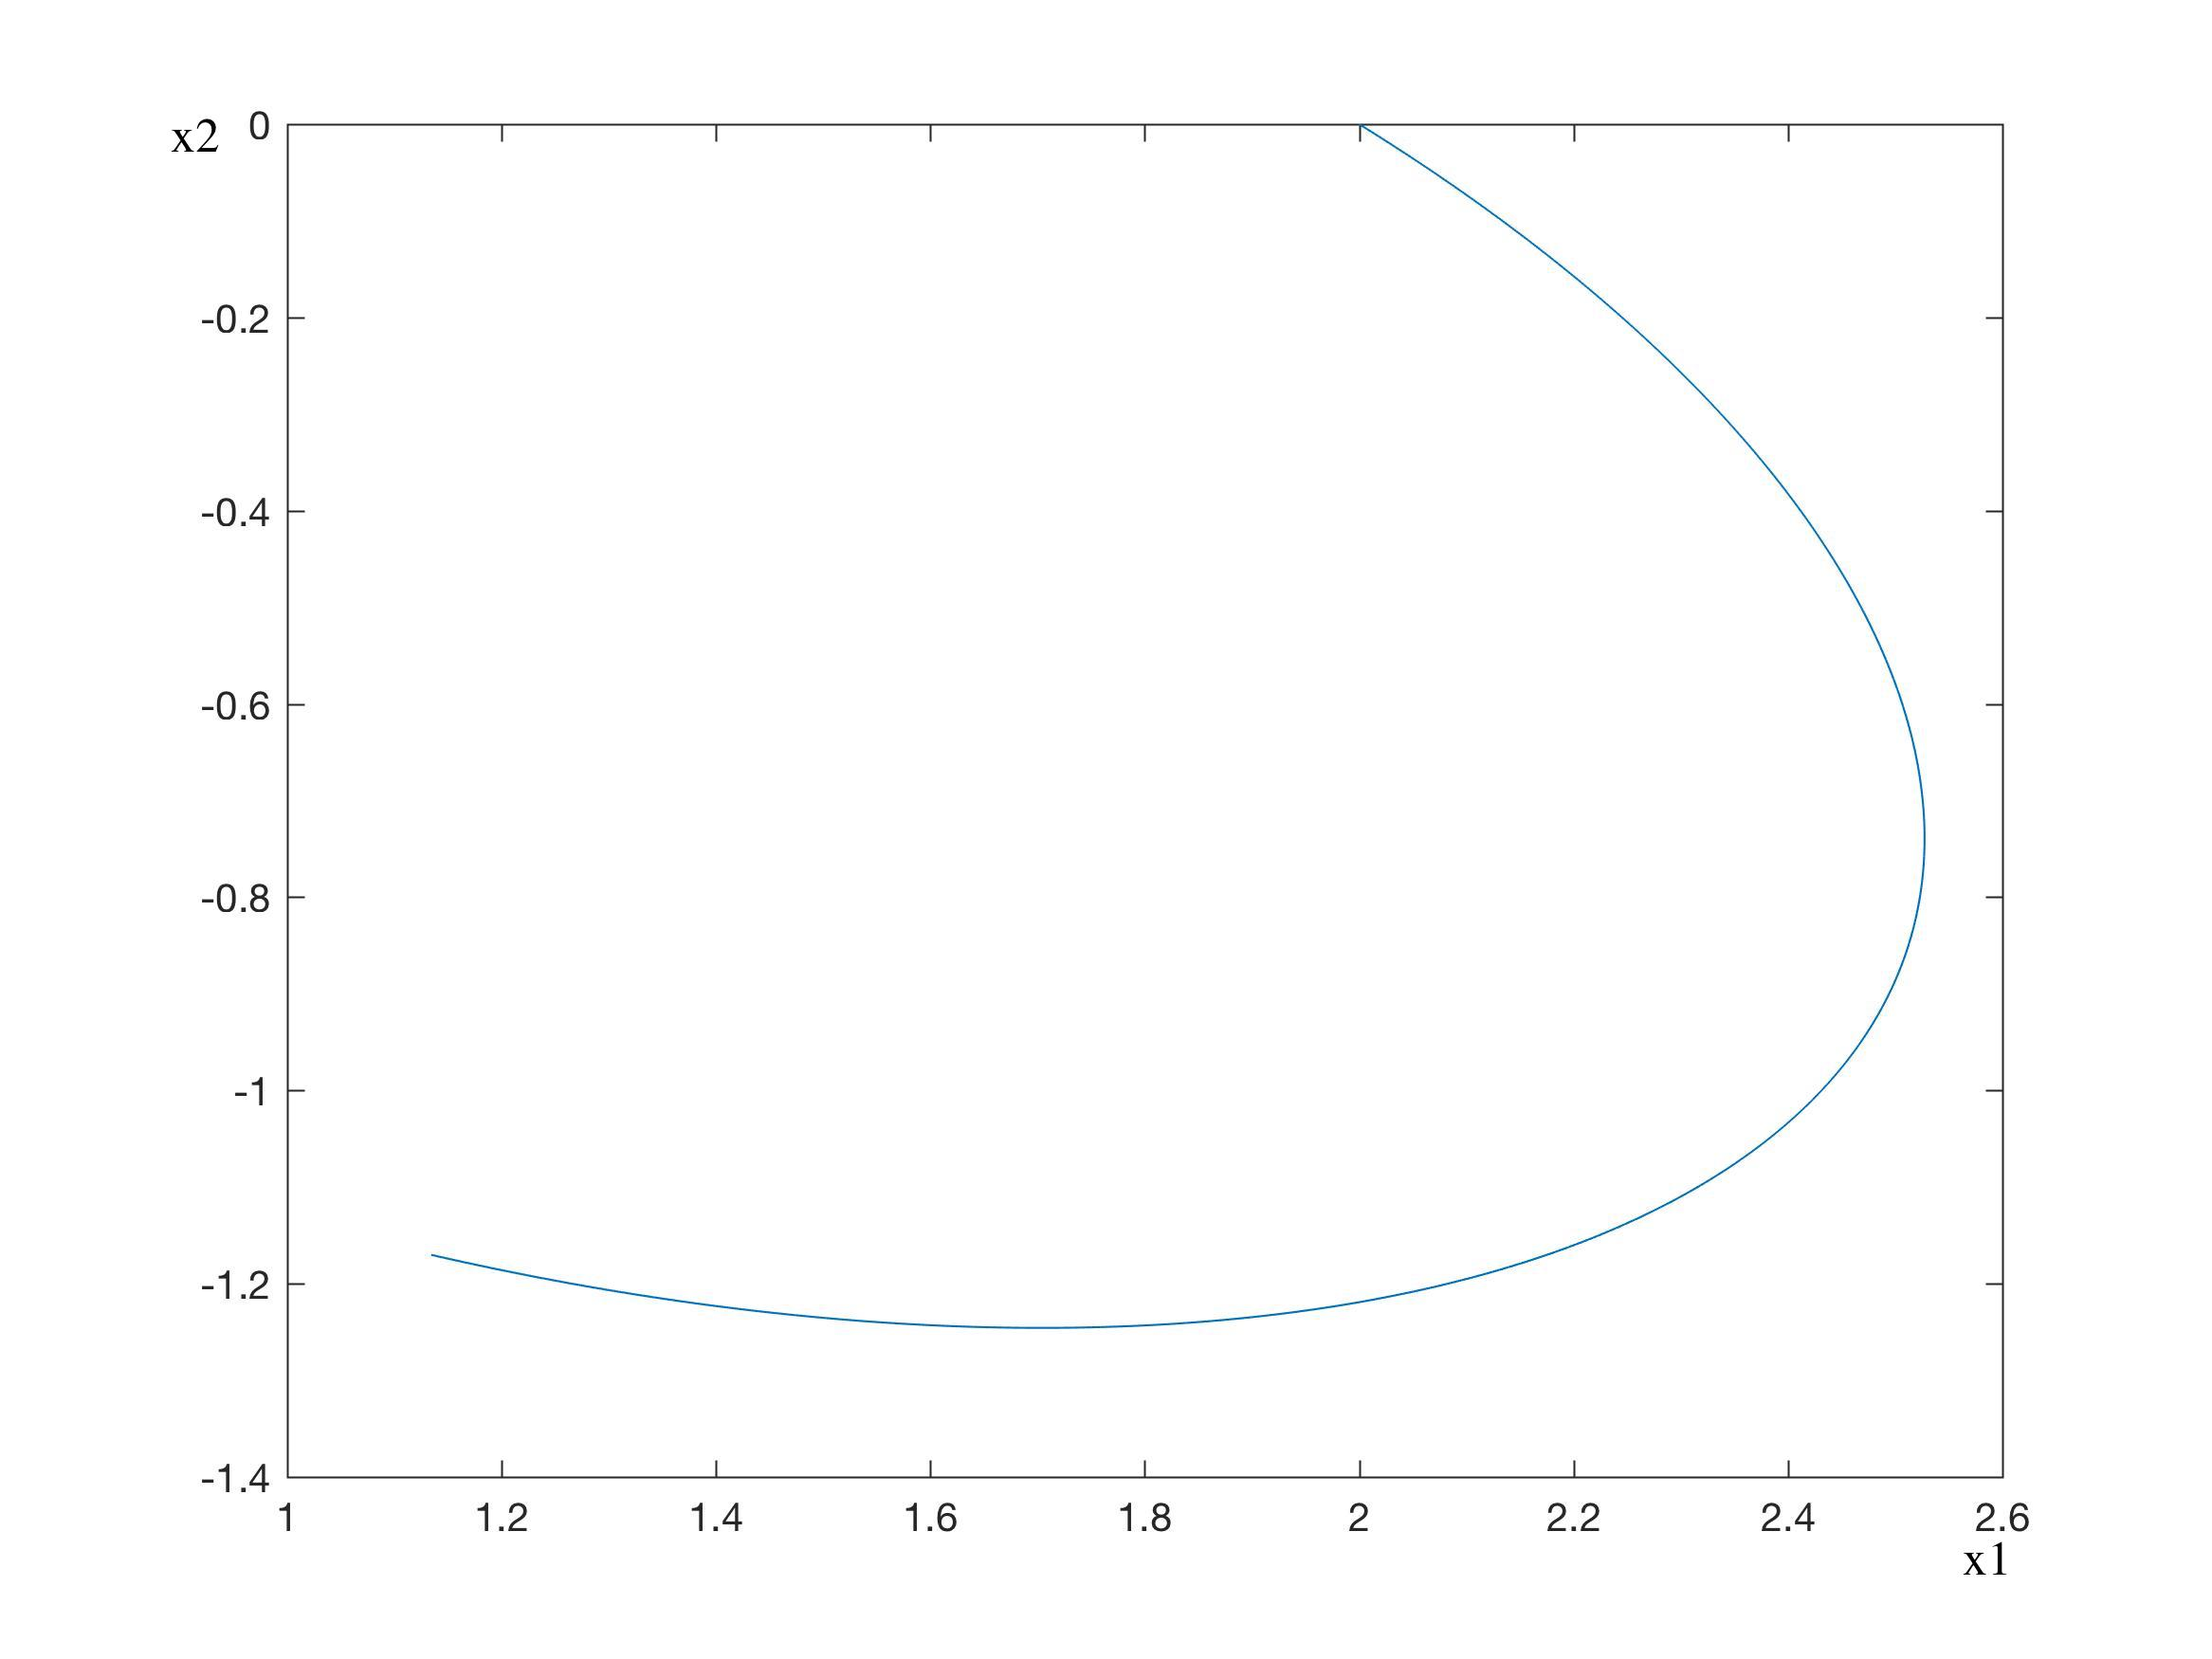
\includegraphics[width=0.7\textwidth]{8}
	\caption{Результат работы}
	\label{gr1}
\end{figure}

\section*{Предельные циклы в системе Эквейлера}
\addcontentsline{toc}{section}{Предельные циклы в системе Эквейлера}

$$
\begin{cases}
\dot{x}_1=x_3x_2, &x_1(0)=x_4(0), \;x_1(1)=x_4(1),
\\
\dot{x}_2=x_3(-x_1+sin(x_2)), &x_2(0)=0, \;x_2(1)=0,
\\
\dot{x}_3=0, 
\\
\dot{x}_4=0.
\end{cases}	
$$

\noindent При выборе параметра $t_* = 0$, для начального приближения 
$$
p_0 = [2, 0, 2\pi, 2].
$$


\begin{figure}[H]
	\centering
	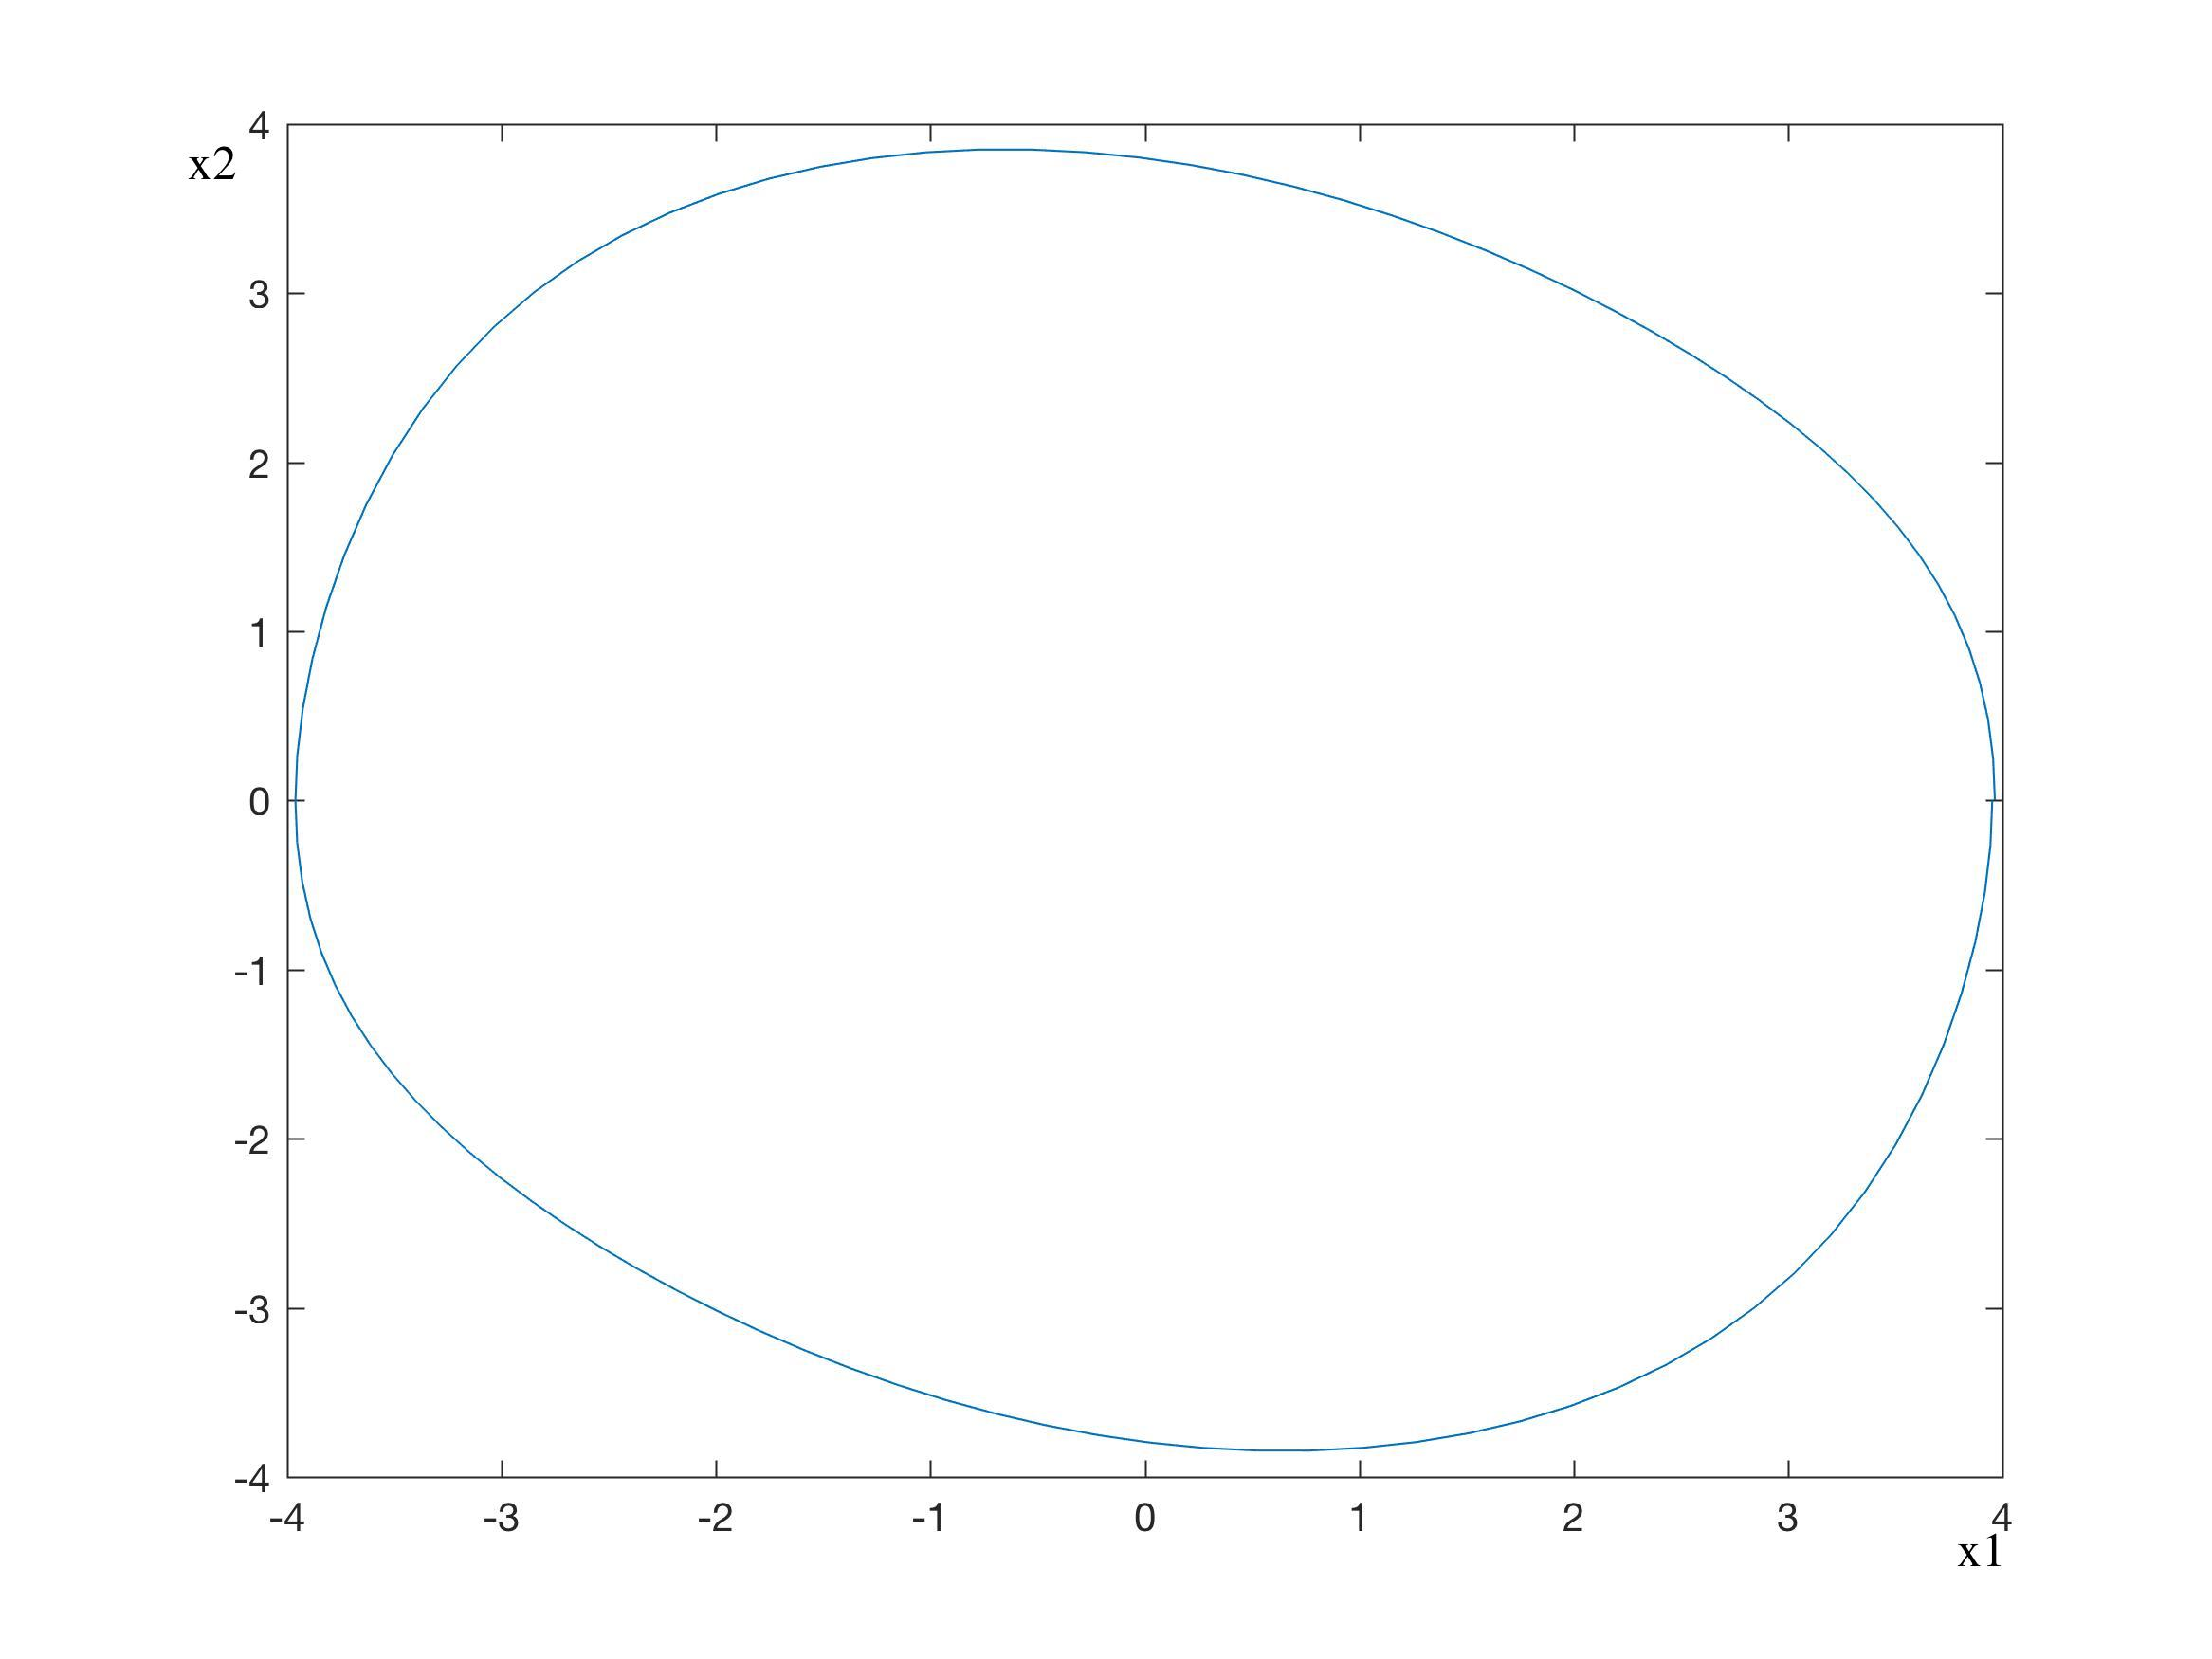
\includegraphics[width=0.7\textwidth]{9}
	\caption{Результат работы}
	\label{gr1}
\end{figure}


\section*{Функционал типа "энергия" для трёхкратного интегратора}
\addcontentsline{toc}{section}{Функционал типа "энергия" для трёхкратного интегратора}

$$
\begin{cases}
\dot{x}_1=x_2,
\\
\dot{x}_2=x_3,
\\
\dot{x}_3=\frac{1}{2}(\sqrt{\nu + (x_6+1)^2}-\sqrt{\nu + (x_6-1)^2}), 
\\
\dot{x}_4=0,
\\
\dot{x}_5=-x_4,
\\
\dot{x}_6=-x_5.
\end{cases}	
$$

\noindent При выборе параметров $t_* = 3.275, \; \nu = 10^{-10}$, для начального приближения 
$$
p_0 = [0, 0, 0, -2.9850435834, 4.8880088678, -2.9083874537].
$$


\begin{figure}[H]
	\centering
	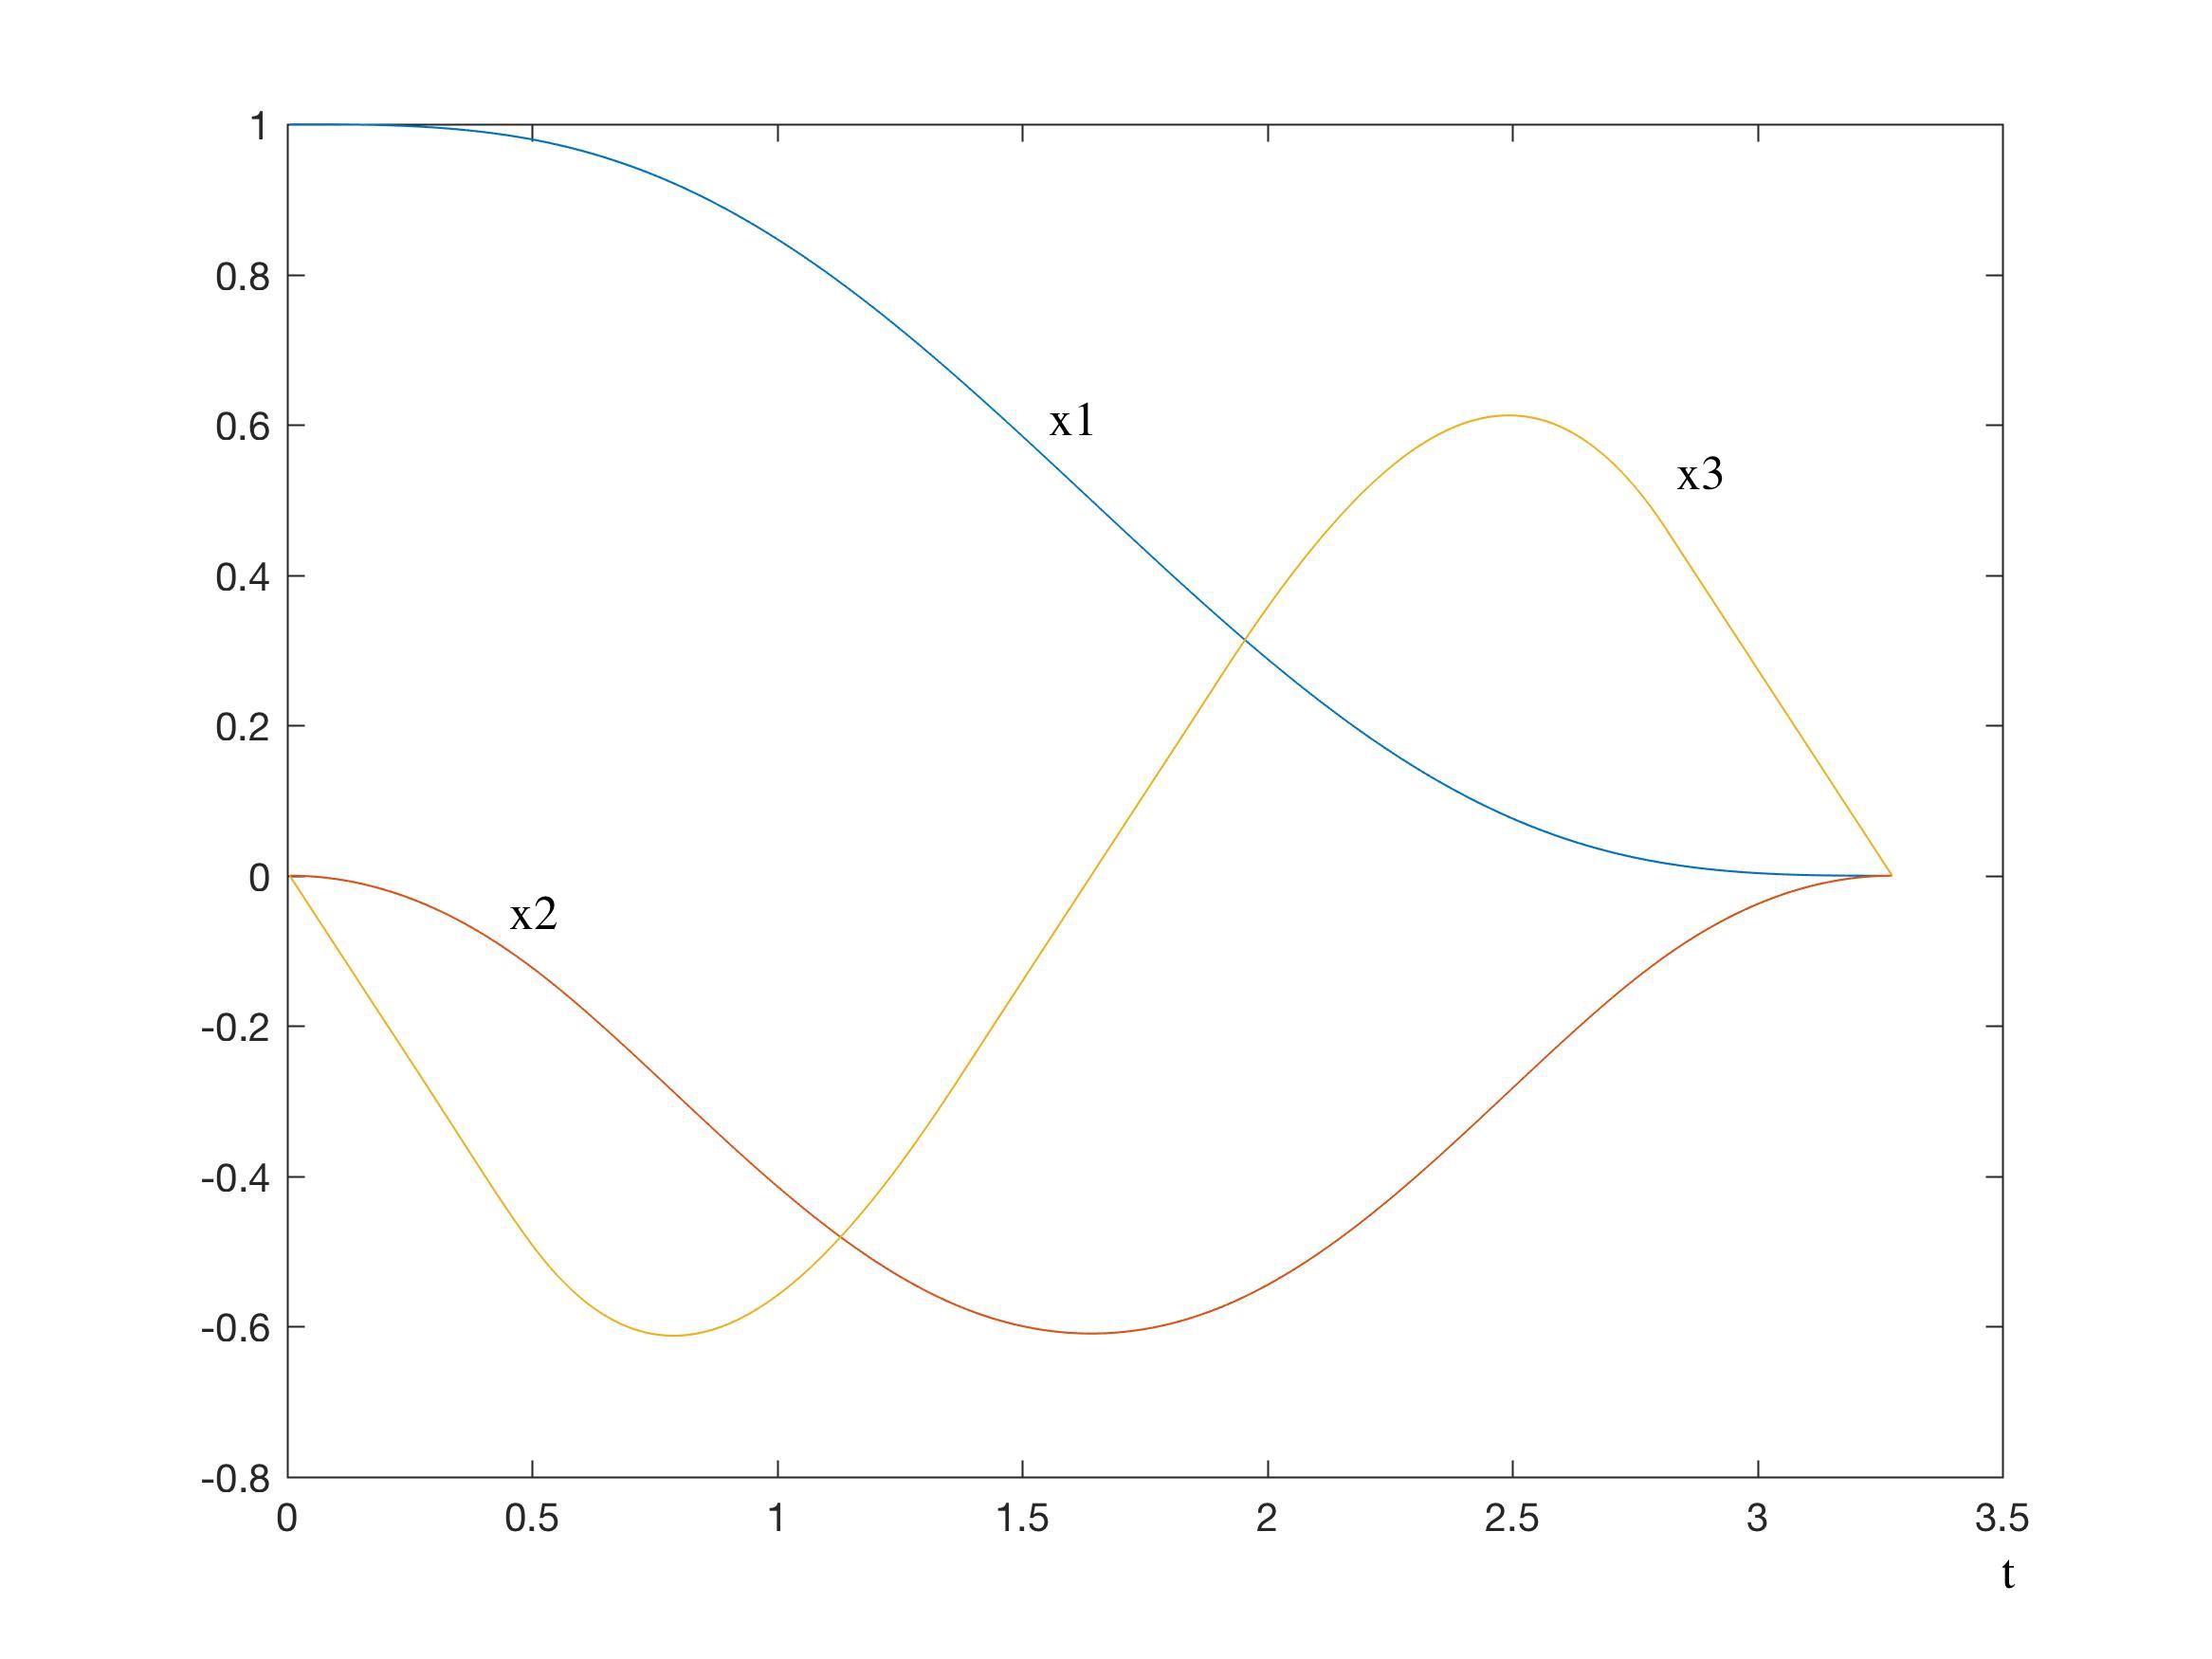
\includegraphics[width=0.7\textwidth]{10}
	\caption{Результат работы}
	\label{gr1}
\end{figure}

\chapter*{Снимки работы программы}
\addcontentsline{toc}{chapter}{Снимки работы программы}

\begin{figure}[h]
	\centering
		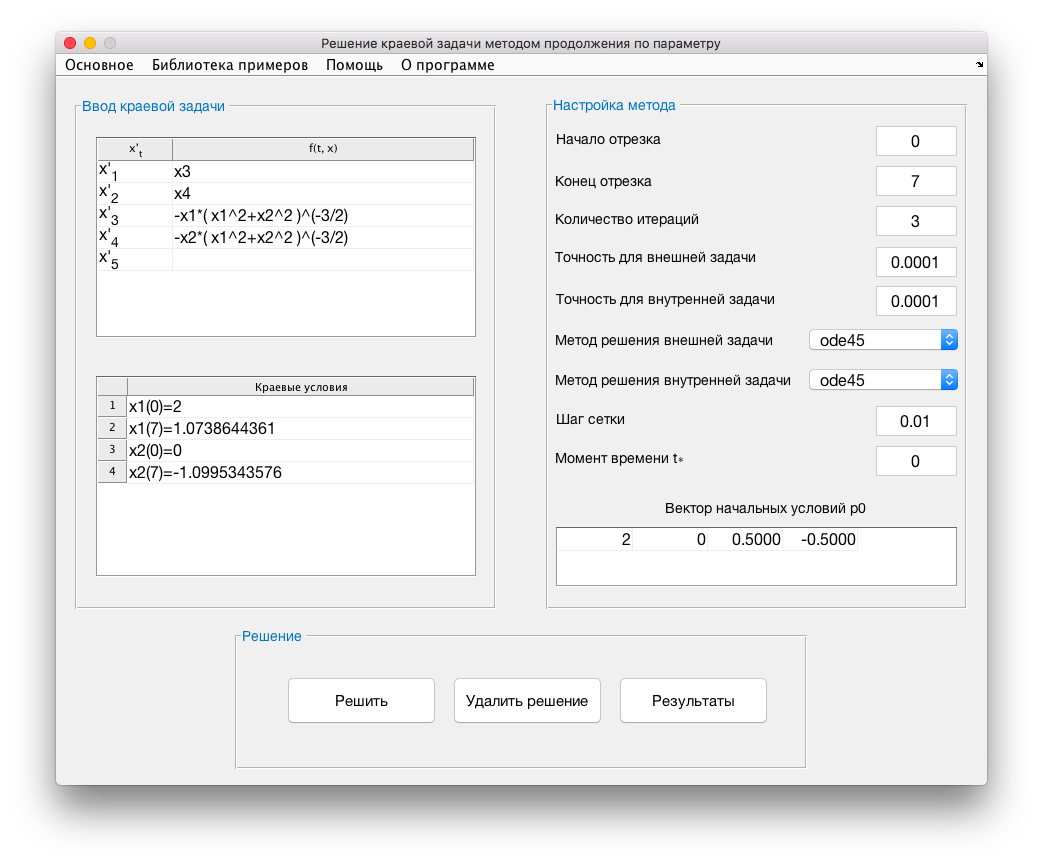
\includegraphics[width=0.9\textwidth]{1}
		\caption{Основное окно}
		\label{gr1}
\end{figure}

\begin{figure}[h]
	\centering
	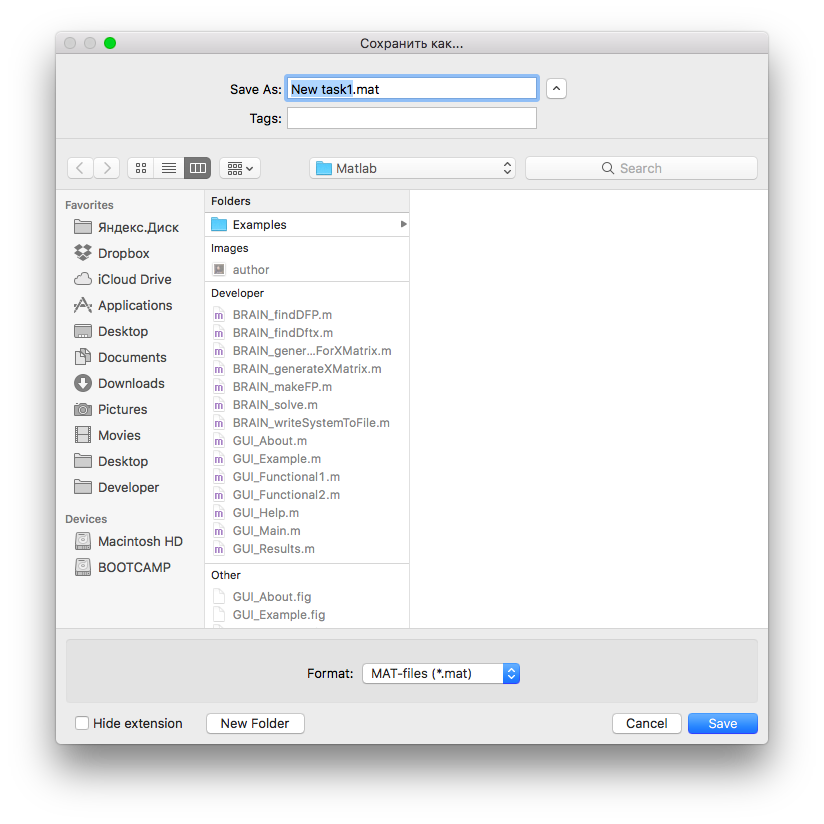
\includegraphics[width=0.9\textwidth]{2}
	\caption{Окно сохранения}
	\label{gr1}
\end{figure}

\begin{figure}[h]
	\centering
	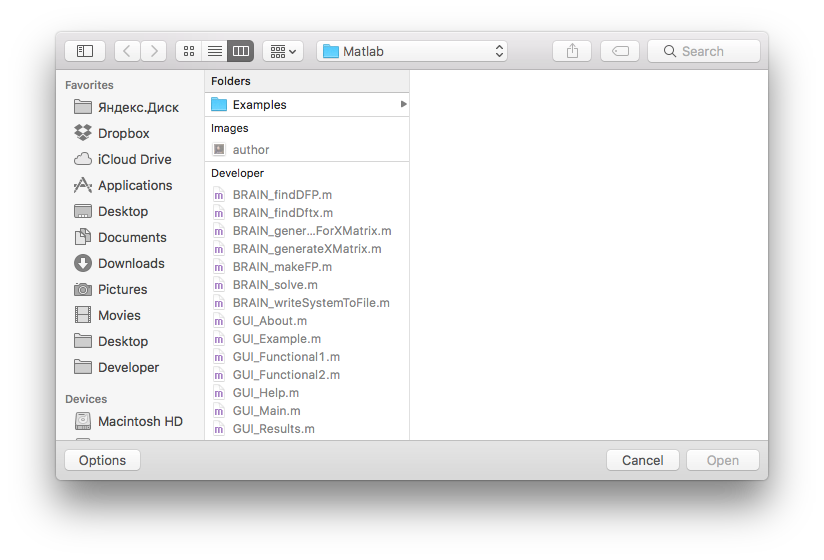
\includegraphics[width=0.9\textwidth]{3}
	\caption{Окно открытия}
	\label{gr1}
\end{figure}

\begin{figure}[h]
	\centering
	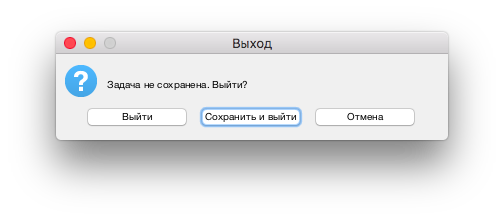
\includegraphics[width=0.9\textwidth]{4}
	\caption{Окно с предупреждением при выходе}
	\label{gr1}
\end{figure}

\begin{figure}[h]
	\centering
	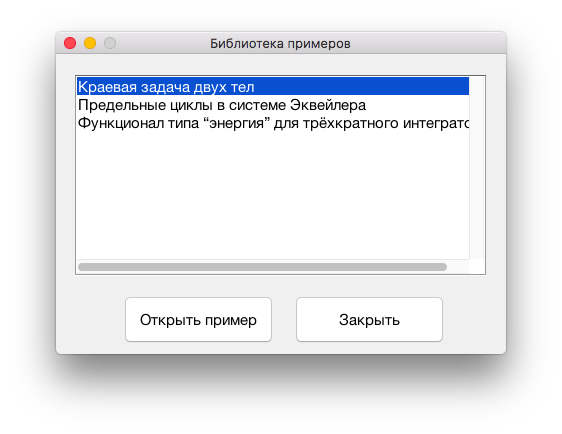
\includegraphics[width=0.9\textwidth]{5}
	\caption{Окно с библитекой примеров}
	\label{gr1}
\end{figure}

\begin{figure}[h]
	\centering
	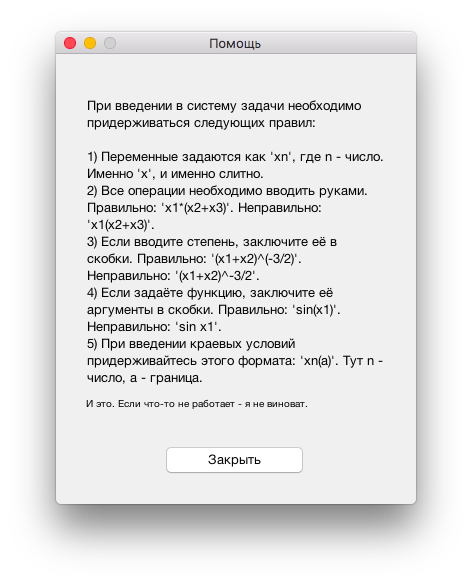
\includegraphics[width=0.7\textwidth]{6}
	\caption{Окно "Помощь"}
	\label{gr1}
\end{figure}

\begin{figure}[h]
	\centering
	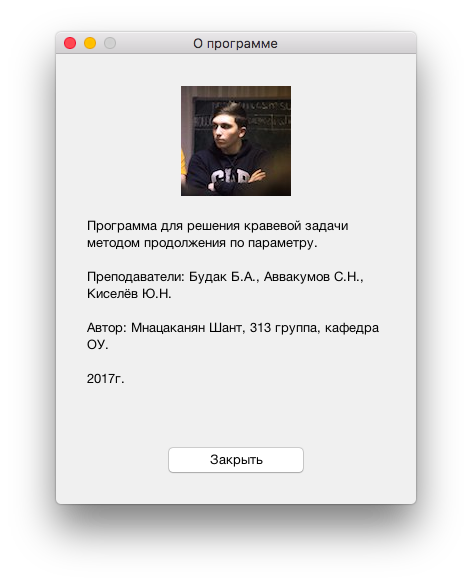
\includegraphics[width=0.7\textwidth]{7}
	\caption{Окно "О программе"}
	\label{gr1}
\end{figure}

\chapter*{Описание математических вычислений}
\addcontentsline{toc}{chapter}{Описание математических вычислений}

Все вычисления выполнены согласно алгоритму, описанному в учебном пособии [5].
\newline 
\newline
\noindent\textit{Файл BRAIN\_solve.m}

\begin{lstlisting}
function solve = BRAIN_solve(inputTaskTableData, conditionsTableData, segBegin, segEnd, stepsCount, accuracyExternal, accuracyInternal, solvingMethodForInternalTask, stepSize, solvingMethodForExternalTask, timeOfT, initialVectorTableData)

%§\mcommentfont\text{Все необходимые данные передаются в функцию}§

ftx = inputTaskTableData; §\mcommentfont\text{Извлекаем краевую задачу}§

dftx = BRAIN_findDftx(ftx); %§\mcommentfont\text{Находим производную}§
XMatrix = BRAIN_generateXMatrix(size(ftx, 1)); %§\mcommentfont\text{Генерируем матрицу Х}§
initConditionForXMatrix = BRAIN_generateInitConditionForXMatrix(size(ftx, 1))'; %§\mcommentfont\text{Генерируем начальные значения для матрицы Х}§
initConditionsForInternalTask = [initialVectorTableData initConditionForXMatrix]; %§\mcommentfont\text{Объединяем вектор начальных значений и начальные значения для матрицы Х}§
DX = dftx*XMatrix; %§\mcommentfont\text{Формируем внутреннюю задачу}§

strDX = reshape(strDX, [n*n, 1]);
toFile = [ftx; strDX];
BRAIN_writeSystemToFile(toFile); %§\mcommentfont\text{Записываем задачу в файл}§
charFP = conditionsTableData;
FP = BRAIN_makeFP(charFP, segBegin, segEnd); %§\mcommentfont\text{Получаем} $\Phi(p)$§
p0 = initialVectorTableData;

for i = 1:stepsCount
	steps = 1/stepSize;
	for j = 0:stepSize:(1-stepSize)
		switch solvingMethodForInternalTask %§\mcommentfont\text{Выбираем метод решения для внутренней задачи}§
			case 1
				if timeOfT == segBegin
					[T, X] = ode45(@systemTemp, [segBegin:internalTaskStepSize:segEnd], initConditionsForInternalTask, odeset('RelTol', accuracyInternal));
				elseif timeOfT == segEnd
					[T, X] = ode45(@systemTemp, [segEnd:-internalTaskStepSize:segBegin], initConditionsForInternalTask, odeset('RelTol', 	accuracyInternal));
					T = T(end:-1:1, :);
					X = X(end:-1:1, :);
				else 
					[T1, X1] = ode45(@systemTemp, [timeOfT:-internalTaskStepSize:segBegin], initConditionsForInternalTask, odeset('RelTol', accuracyInternal));
					[T2, X2] = ode45(@systemTemp, [timeOfT:internalTaskStepSize:segEnd], initConditionsForInternalTask, odeset('RelTol', accuracyInternal));
					T = [T1(end:-1:2); T2];
					X = [X1(end:-1:2, :); X2];
				end
			case 2
				...
			case 3
				...
			case 4
				...
			case 5
				...
			case 6
				...
		end

		n = size(FP, 1);

		XAP = X(1, n+1:end); %§\mcommentfont\text{Находим} $X(a, p)$§
		XAP = reshape(XAP, [n n]);
		XBP = X(end, n+1:end); %§\mcommentfont\text{Находим} $X(b, p)$§
		XBP = reshape(XBP, [n n]);

		XP0 = num2cell([X(1, 1:n) X(end, 1:n)]);

		FP0 = subs(FP(:, 1), symArray1, XP0); %§\mcommentfont\text{Находим} $\Phi(p_0)$§

		DRXA = jacobian(FP, symArray2); %§\mcommentfont\text{Находим} $R'_x$§
		DRXB = jacobian(FP, symArray3); %§\mcommentfont\text{Находим} $R'_y$§

		DRXA = subs(DRXA, symArray1, XP0);
		DRXB = subs(DRXB, symArray1, XP0);

		switch solvingMethodForExternalTask %§\mcommentfont\text{Выбираем метод решения для внешней задачи}§ 
			case 1
				[mu, p] = ode45(@BRAIN_findDFP, [j (j+stepSize)], p0, odeset('RelTol', accuracyExternal));
			case 2
				...
			case 3
				...
			case 4
				...
			case 5
				...
			case 6
				...
			case 7
				p = (BRAIN_findDFP*stepSize+p0')';
		end
		
		p0 = p(end, :);
		initConditionsForInternalTask = [p0 initConditionForXMatrix];
	end
end

solve = [T(:, :), X(:, 1:n)]; %§\mcommentfont\text{Записываем результат}§

end
\end{lstlisting}


\begin{thebibliography}{0}

\bibitem{1}
Википедия. \emph{ru.wikipedia.org}.

\bibitem{2} С. М. Львовский
\emph{Набор и вёрстка в системе \LaTeX{}} // Издательство Макс Пресс, 2003.

\bibitem{3}
Встроенный <<Help>> среды \emph{Matlab}. 

\bibitem{4}
Официальный <<Help>>. \emph{matlab.com}.

\bibitem{}
Ю.Н. Киселёв, С.Н. Аввакумов, М.В. Орлов \emph{Оптимальное управление. Линейная теория и приложения} // 2007, Издательский отдел факультета ВМК МГУ имени М.В. Ломоносова, 270.

\end{thebibliography}

\end{document}